\subsection{Wagasci module}
To demonstrate the performance of the Wagasci module and also to study the neutrino interaction,
the first Wagasci module was installed at the on-axis position, in front of the T2K INGRID horizontal center module
in 2016.
The INGRID module is made of iron plates and segmented plastic scintillator bars.
It's cross sectional size viewed from the beam direction is 1~m$\times$1~m.
The charged current interactions in the Wagasci module are selected by requiring a muon track candidate
in the INGRIRD modules.
Here, we describe the performance of the Wagasci module evaluated at this T2K on-axis measurement.
Figure~\ref{fig:wmlight} shows the light yeild of channels for muons produced by the interaction of neutrinos
in the hall wall.
The light yield is sufficiently hgih to get good hit efficieincy.  
\begin{figure}[tbh]
\begin{center}
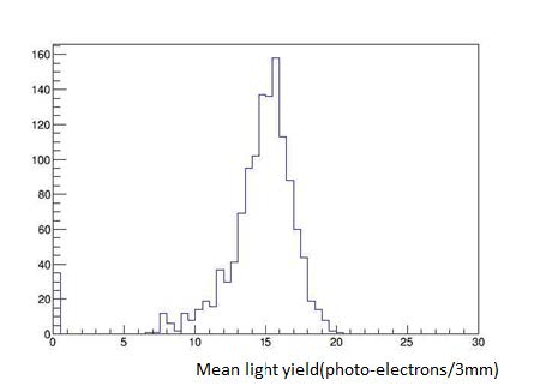
\includegraphics[width=0.5\linewidth]{fig/wmlight.pdf}
\end{center}
\caption{Light yield of channels for muons produced by the interaction of neutrinos
  in the hall wall.
}
\label{fig:wmlight}
\end{figure}
The tracking efficiency in 2-dimentional projected plane was evalualted by comparing the reconstructed track
in the Wagasci module and the INGRID module and shown in Fig.\ref{fig:wmefficiency}.
Note that that the tracking efficinecy for high angle ($>70\deg$) is not evaluated because of the acceptance
of the INGRID module, not because of the limitation of the Wagasci module.
\begin{figure}[tbh]
  \begin{center}
   \begin{subfigure}{0.48\textwidth}
     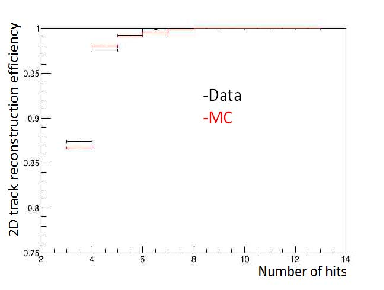
\includegraphics[width=\linewidth]{fig/wmeffvshit.pdf}
    \end{subfigure}
  \begin{subfigure}{0.48\textwidth}
      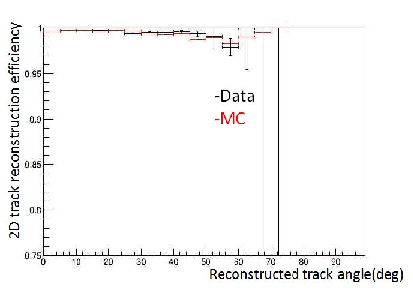
\includegraphics[width=\linewidth]{fig/wmeffvsangle.pdf}
    \end{subfigure}    
    \end{center}
  \caption{2D track reconstruction efficiency as a function of number of hits (left) and track angle (right).
  Here the track angle is the one reconstructed by the INGRID module.}
\label{fig:wmefficiency}
\end{figure}

